%%%%%%%%%%%%%%%%%%%%%%%%%%%%%%%%%%%%%%%%%%%%%%%%%%%%%%%%%%%%%%%%%%%%%%%%%%%%%%%%%
%																				%
%                                ELEN4020.tex    			    				%
%						    	Emma Clark(1088496) 							%
%                               Jason Smit (709363)		        				%
%						      Isabel Tollman (728359)           				%
%                                                                   		    %
%                                                                               %
%																				%
%%%%%%%%%%%%%%%%%%%%%%%%%%%%%%%%%%%%%%%%%%%%%%%%%%%%%%%%%%%%%%%%%%%%%%%%%%%%%%%%%
\documentclass[10pt,onecolumn]{witseiepaper}
\pagenumbering{arabic} %set the style of numbering

\usepackage[none]{hyphenat}
\usepackage{flushend}
\usepackage{rotating} %
\usepackage{url} %for url's in the reference
\usepackage[square,comma,numbers,sort&compress]{natbib} %for referencing very important
\usepackage{balance} %balance the last page
\usepackage{amsmath} %math package
\usepackage{xr} %Reference appendix

% for putting code into the report : Looks really good
%%%%%%%%%%%%%%%%%%%%%%%%%%%%%%%%%%%%%%%%%%%%%%%%%%%%%%%%%%%%%%%%%%%%%%%%%%%%%%%%%
\usepackage{listings} 															%
\usepackage{color} 		%
																				%
\definecolor{dkgreen}{rgb}{0,0.6,0}												%
\definecolor{gray}{rgb}{0.5,0.5,0.5}											%
\definecolor{mauve}{rgb}{0.58,0,0.82}											%
																				%
\lstset{frame=tb,																%
  language=C,																%
  aboveskip=3mm,																%
  belowskip=3mm,																%
  showstringspaces=false,														%
  columns=flexible,																%
  basicstyle={\small\ttfamily},													%
  numbers=none,																	%
  numberstyle=\tiny\color{gray},												%			
  keywordstyle=\color{blue},													%
  commentstyle=\color{dkgreen},													%
  stringstyle=\color{mauve},													%
  breaklines=true,																%
  breakatwhitespace=true,														%
  tabsize=3																		%
}																				%
%%%%%%%%%%%%%%%%%%%%%%%%%%%%%%%%%%%%%%%%%%%%%%%%%%%%%%%%%%%%%%%%%%%%%%%%%%%%%%%%%


		\pdfinfo{
		/Title ()
		/Author (Jason R. Smit)
		/CreationDate (D:201711040830)
		/ModDate (D:201711052000)	
		/Subject (FINAL DRAFT)
		/Keywords ()
		}%needed to put information into a pdf discription file

%%%%%%%%%%%%%%%%%%%%%%%%%%%%%%%%%%%%%%%%%%%%%%%%%%%%%%%%%%%%%%%%%%%%%%%%%%%%%%%

%\usepackage{siunitx}
\usepackage{float}


%%%%%%%%%%%%%%%%%%%%%%%%%%%%%%%%%%%%%%%%%%%%%%%%%%%%%%%%%%%%%%%%%%%%%%%%%%%%%%%
\begin{document}
%\begin{titlepage}

\title{\centering \textbf{{ELEN4020-LAB1}}}

\author{\centering {{Emma Clark \\ Jason Smit \\ Isabel Tollman}
{ \\ \normalfont \textit{School of  Electrical \& Information Engineering.} \\
\textit{University of the
Witwatersrand}\\
Private Bag 3, 2050, Johannesburg, South Africa \\}}}
%\thanks{School of  Electrical \& Information Engineering. University of the
%Witwatersrand, Private Bag 3, 2050, Johannesburg, South Africa}


%%%%%%%%%%%%%%%%%%%%%%%%%%%%%%%%%%%%%%%%%%%%%%%%%%%%%%%%%%%%%%%%%%%%%%%%%%%%%%%
% 
\abstract{This report presents the procedure for tensor multiplication and addition of rank 2 and 3. The rank 3 tensor is built using the methods used in rank 2 tensors.}

\keywords{2D, 3D, Tensor, pseudocode}


\maketitle
\thispagestyle{empty}\pagestyle{empty}
%\end{titlepage}

%%%%%%%%%%%%%%%%%%%%%%%%%%%%%%%%%%%%%%%%%%%%%%%%%%%%%%%%%%%%%%%%%%%%%%%%%%%%%%%
%

\section{INTRODUCTION} 
This report seeks to investigate tensor operations carried out on rank 3 tensors. The rank 2 tensors procedures and the pseudocode required to achieve the procedures are presented. Using the basis of rank 2 tensors, rank 3 tensor operations are demonstrated along with pseudocode implementation. Each of the procedures is further implemented using C++ from the basis of the pseudocode.  
\section{2D TENSOR ADD}
The addition of two 2-dimensional tensors is congruent to 2 dimensional matrices. This therefore requires using element-by-element addition, as shown in Equation \ref{2d-add-eqn}. Algorithm 1 displays the pseudo-code used to calculate the addition of two N$\times$N matrices.

\begin{align}
C_{ij} = A_{ij} + B_{ij} \label{2d-add-eqn}
\end{align}
\subsection{Code}
\begin{figure}[H]
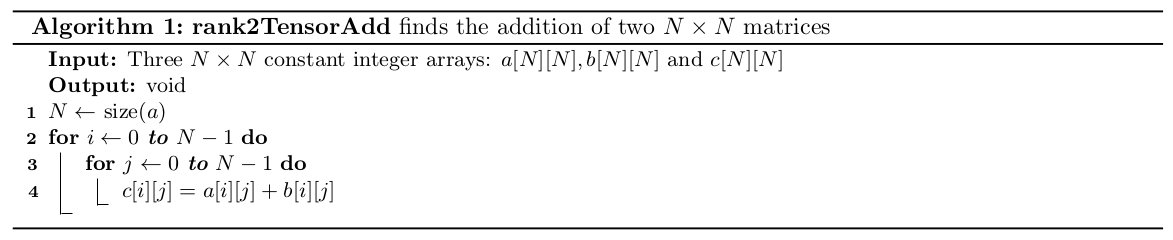
\includegraphics[width=\textwidth]{build/Algo1.png}
\end{figure}
\section{2D TENSOR MULTIPLY}
The multiplication of rank 2 tensors is equivalent to 2-dimensional matrix multiplication which is achieved by performing the dot product on the respective
rows and columns, as illustrated in Equation \ref{2d-mult-eqn}. Algorithm 2 shows the pseudo-code used to multiply two N$\times$N matrices.
\begin{align}
C_{ij} = \sum_{k} A_{ij} \times B_{ij} \label{2d-mult-eqn}
\end{align}

\subsection{Code}
\begin{figure}[H]
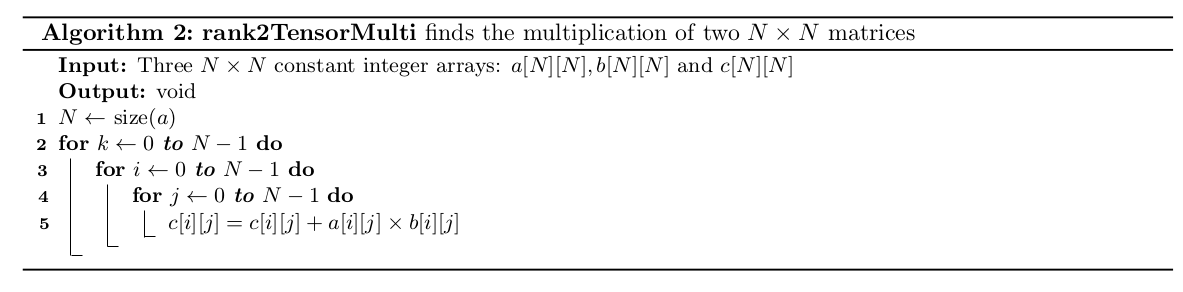
\includegraphics[width=\textwidth]{build/Algo2.png}
\end{figure}
\section{3D TENSOR ADD}
Using the rank 2 tensors as a basis, when a third rank is added the addition follows the same procedure, however the additional rank corresponds to an additional vertex of summation. The addition is achieved using element-by-element addition, similar to a 2D array. The difference is only the inclusion of the additional dimension. Algorithm 3 shows the pseudo-code used to sum two N$\times$N$\times$N matrices.
\subsection{Code}
\begin{figure}[H]
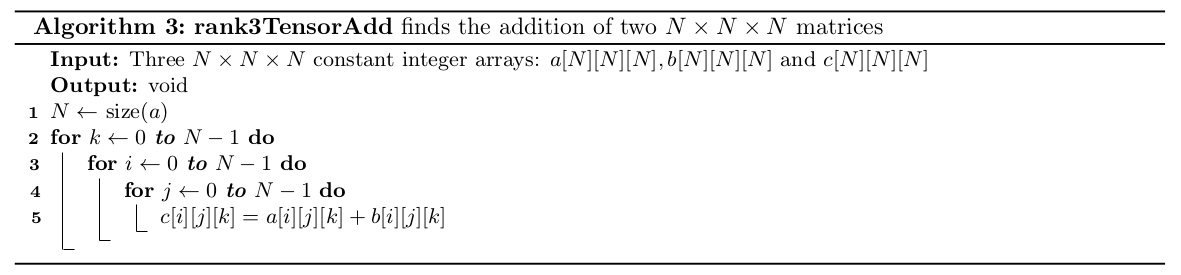
\includegraphics[width=\textwidth]{build/Algo3.png}
\end{figure}
\section{3D TENSOR MULTIPLY}
The multiplication of two 3-dimensional arrays makes use of 2-dimensional matrix multiplication as a basis. The $\text{i}^\text{th}$row-plane of array A and the $\text{j}^\text{th}$ column-plane of array B are multiplied using traditional 2-dimensional matrix multiplication shown in Algorithm \ref{2d-mult-eqn}. The result is the $\text{k}^\text{th}$ layer-plane of array C. Algorithm 4 shows the pseudo-code used to multiply two N$\times$N$\times$N matrices. This can be visualised as is seen in figure \ref{3D}
\begin{figure}
\centering
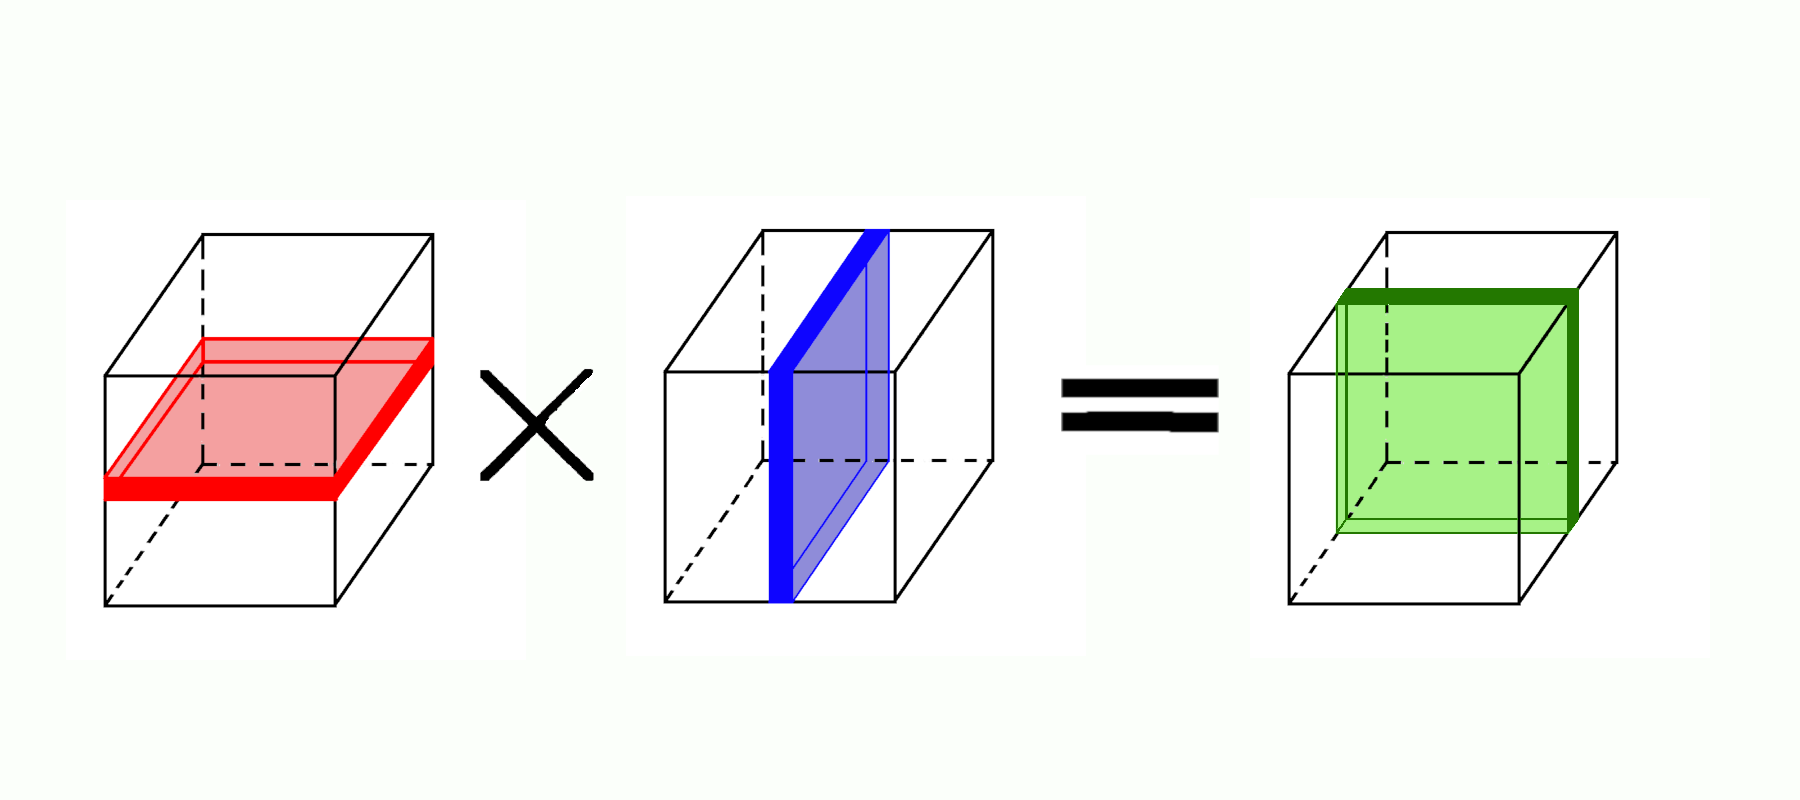
\includegraphics[scale=0.5]{build/3Dmult.png}
\caption{Visualisation of a tensors multiplication of rank 3}
\label{3D}
\end{figure}
\subsection{Code}
\begin{figure}[H]
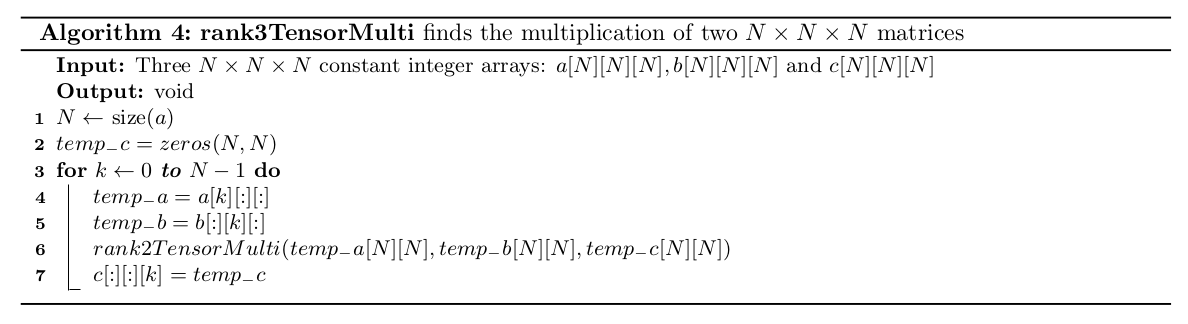
\includegraphics[width=\textwidth]{build/Algo4.png}
\end{figure}
\section{IMPLEMENTATION}
The preceding sections' pseudocode is implemented using c++. The code generated performs as detailed by the pseudocode and is accessible via the public github link \url{https://github.com/IsabelTollman/ELEN4020A_Group7/tree/Code} under the `\emph{Code}' branch.

%%%%%%%%%%%%%%%%%%%%%%%%%%%%%%%%%%%%%%%%%%%%%%%%%%%%%%%%%%%%%%%%%%%%%%%%%%%%%%%%
\section{CONCLUSIONS}
The formation of rank 3 tensor operations is based on the rules of rank 2 tensors, with the addition of the multiple iterations present in the additional dimension. 

\cite{1}
 
%%%%%%%%%%%%%%%%%%%%%%%%%%%%%%%%%%%%%%%%%%%%%%%%%%%%%%%%%%%%%%%%%%%%%%%%%%%%%%%
%\clearpage %On a newpage
%\onecolumn
\bibliographystyle{build/witseie}
\bibliography{build/Ideal}

%{\tiny \vfill \hfill \today \hspace{5mm} witseie-paper-2003.\TeX}


%%%%%%%%%%%%%%%%%%%%%%%%%%%%%%%%%%%%%%%%%%%%%%%%%%%%%%%%%%%%%%%%%%%%%%%%%%%%%%%%%%%%%%%%%%%%%%%%%%%%%%%%%%%%%%%%%%%%%%%%%%%%%%%%%%%%%%%%%%%
\end{document}

" vim: ts=4
" vim: tw=78
" vim: autoindent
" vim: shiftwidth=4
